\documentclass[journal]{IEEEtran}
\usepackage{cite}
\usepackage[cmex10]{amsmath}
\usepackage{graphicx}
\DeclareGraphicsExtensions{.pdf,.png,.jpg,.eps}
\usepackage{algorithm}
\usepackage{algorithmic}
\usepackage[tight,footnotesize]{subfigure}
\usepackage{tikz}
\usetikzlibrary{shapes,arrows}
\usepackage{subfigure}
\usepackage{epstopdf}
%\usepackage{caption}

\hyphenation{Ala-mouti}

\begin{document}

\title{Simulation of an Adaptive Cooperative Diversity Algorithm for Ad-hoc Networks}

\author{\IEEEauthorblockN{Spencer Chan and Caleb Zulawski}\\
\IEEEauthorblockA{Albert Nerken School of Engineering\\
The Cooper Union for the Advancement of Science and Art\\
New York, New York}}

\maketitle


\begin{abstract}
We implement a cross-layer design utilizing a cyclic redundancy check (CRC) on the transport layer to detect poor channel state and Alamouti's space-time block code on the link layer for retransmission.
Retransmissions are performed with cooperative diversity, utilizing inactive nodes in a virtual antenna array.
Diversity nodes are selected at the transport layer, rather than the link layer, reducing the channel quality estimation to a CRC.
We also simulate different methods of selecting retransmission nodes by taking into account likelihood of retransmission.
We find that utilizing cooperative diversity significantly increases throughput, especially in shadow fading environments where all nodes do not have line of sight channels to all other nodes.
\end{abstract}

\begin{keywords}
Cooperative diversity, cross-layer design, CRC, Alamouti's code, ad-hoc networks
\end{keywords}

\section{Introduction}
\IEEEPARstart{W}{ireless} ad-hoc networks have recently become a topic of research as they can be deployed quickly in locations lacking the infrastructure required for typical wireless networks.

Like any wireless network, ad-hoc networks would benefit greatly from the diversity advancements made in the last couple decades.

Compared to the transmitters and receivers in traditional wireless networks, the nodes in an ad-hoc network may be much smaller and possibly mobile.
This discourages the use of many techniques for increasing capacity, most notably the use of multiple antennas at the transmitter for obtaining a diversity gain.
A diversity strategy is proposed in \cite{4686273} that creates a virtual antenna array by utilizing inactive neighboring nodes in transmitting with an orthogonal space-time block code.

The key measurement in this paper is throughput, as high throughput in a wireless network is the defining metric of a good connection.  Therefore, we will attempt to validate the results by means of comparing the throughput of a system with that of an identical system implementing an adaptive cooperative diversity scheme. Throughput in this paper is defined as the ratio of the number of packets successfully transmitted to the total number of packets transmitted, under the assumption that the overhead of obtaining diversity nodes is insignificant compared to the transmission time of a packet.

\section{Adaptive Cooperative Diversity}
A cooperative diversity algorithm was described in \cite{4686273} and was used as a basis for the simulation.

\subsection{Diversity Strategy}
If we consider an ad-hoc network consisting of many separate devices, it can be assumed that some of these nodes will be idle and available for data transmission.
These inactive nodes can be utilized for transmission with an orthogonal space-time block code.
The source node and nearby inactive nodes can be thought of as a virtual antenna array and can be used to obtain a diversity gain.
To limit unnecessary use of other nodes, the transmission only falls back to cooperative diversity if the destination node fails the CRC from the source-only transmission. A simple implementation of this process can be seen in Figure  \ref{fig:flowchart}.

\tikzstyle{decision} = [diamond, draw, fill=none, 
    text width=4.5em, text badly centered, inner sep=0pt]
\tikzstyle{block} = [rectangle, draw, fill=none, 
    text width=5em, text centered, rounded corners, minimum height=3em]
\tikzstyle{line} = [draw, -latex']

\begin{figure}
	\begin{tikzpicture}[node distance = 2.5cm, auto, font=\scriptsize]
	    \node [block] (direct) {Source node broadcasts data};
	    \node [block, below of=direct, node distance=1.5cm] (crc) {All nodes within range check CRC};
	    \node [decision, below of=crc] (destchk) {Destination node has correct CRC};
	    \node [block, left of=destchk, node distance=3cm] (destack) {Destination node sends ACK};
	    \path [line] (destack) |- (direct);
	    \node [block, below of=destchk] (destnack) {Destination node sends NACK};
	    \node [decision, below of=destnack] (otherschk) {Other nodes have correct CRC};
	    \node [block, below of=otherschk] (candidate) {Choose a candidate and retransmit with Alamouti's code};
	    \node [decision, below of=candidate] (destchk2) {Destination node has correct CRC};
	    \node [block, right of=destchk2] (destnack2) {Destination node sends NACK};
	    \node [block, right of=otherschk] (retx) {Source node must retransmit the packet};
	   
	   
	    \path [line] (direct) -- (crc);
	    \path [line] (crc) -- (destchk);
	    \path [line] (destchk) -- node [near start] {Yes} (destack);
		\path [line] (destchk) -- node [near start] {No} (destnack);
		\path [line] (destnack) -- (otherschk);
		\path [line] (otherschk) -- node [near start] {Yes} (candidate);
		\path [line] (otherschk) -- node [near start] {No} (retx);
		\path [line] (candidate) -- (destchk2);
		\path [line] (destchk2) -| node [near start] {Yes} (destack);
		\path [line] (destchk2) -- node [near start] {No} (destnack2);
		\path [line] (destnack2) -- (retx);
		\path [line] (retx) |- (direct);
	\end{tikzpicture}
	
	\caption{Flowchart of the simulated algorithm.}
	\label{fig:flowchart}
\end{figure}

\subsection{Distance and Shadow Fading Considerations}
Simply picking a diversity node at random from the list of nodes that passed the CRC is not the most efficient method.
Consider the network topology shown in Figure \ref{fig:4x4topology}.
Assume that the circle around node 10 is a building introducing significant shadowing to the channels passing through it.
Consider that node 1 is attempting to transmit data to node 11.
While nodes 2 and 5 will pass the CRC equally often,  a cooperative diversity transmission with node 2 is much more likely to be successful than one with node 5.
The same is true for nodes 3 and 9.
Figure \ref{fig:histogram} contains the results of 1000 packet transmissions where the diversity nodes where chosen from a uniform random distribution.
While nodes 2 and 5 were selected for diversity about the same number of times, node 5 was obviously not a good choice for cooperative diversity.
To account for this, Algorithm \ref{alg1} was developed.
When the node enters the network, it assumes that all nodes have an equal probability of performing a successful transmission as a diversity node.
As transmissions are made, the node keeps track of the probability of transmission and selects the diversity nodes based on which of the diversity candidate nodes has the highest probability of transmission.

\subsection{Simulation}
The simulation was created in MATLAB.  Each node had a transmit power of 100 mW and used 4-QAM modulation at a symbol rate of 1 Msymbols/s.  The carrier frequency was set as 2.4GHz, a common frequency used in the industrial, scientific, and medical (ISM) band.  Channels were assumed to be quasi-static (static over the entire packet) Rayleigh fading channels with free space path loss and the log-distance propagation model for shadowing:
\begin{align*}
\gamma &= 3.0\\
\sigma &= 7.0 \mbox{ dB}\\
X &\sim \mathcal{N}(0,\sigma^2)\\
L &= 10\log_{10}\left(\frac{4\pi d f}{c}\right)^2 + 10\gamma \log_{10} \frac{d}{1000m} + X
\end{align*}
where $L$ is the path loss in dB, $d$ is the distance in meters, and $f$ is the carrier frequency.
The values of $\gamma$ and $\sigma$ were selected to approximate the shadowing as an office building.
The simulation was performed by transmitting 1000 randomly generated 2KB packets at each noise floor value.
The CRC generator polynomial used was for CRC-16, as follows:
\begin{align*}
g(x) = x^{16} + x^{15} + x^{2} + 1
\end{align*}

\begin{figure}
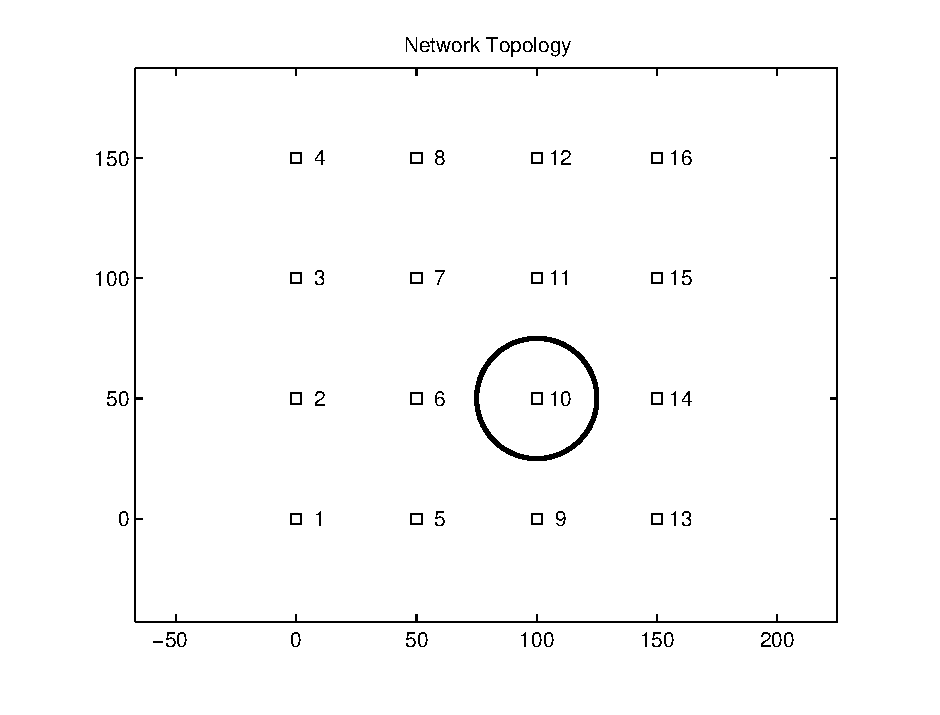
\includegraphics[scale=.6]{figures/4x4topology}
\caption{Topology of a 4x4 grid network.}
\label{fig:4x4topology}
\end{figure}
\begin{figure}
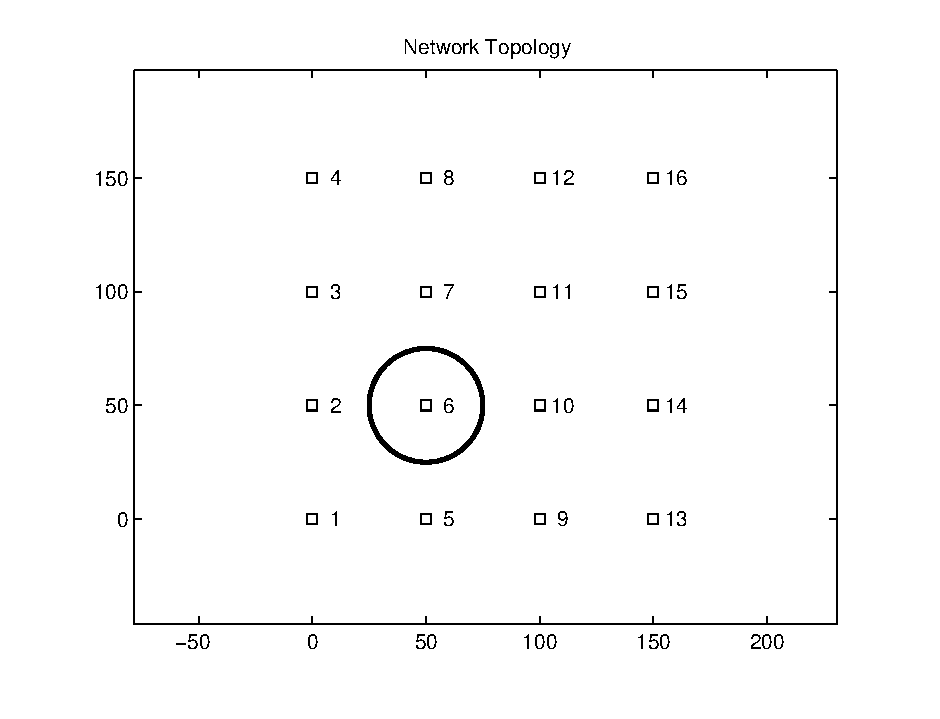
\includegraphics[scale=.6]{figures/4x4topology_shadowing}
\caption{Topology of a 4x4 grid network with shadowing in the path of transmission.}
\label{fig:4x4topologyshadowing}
\end{figure}
\begin{figure*}[ht]
\centering
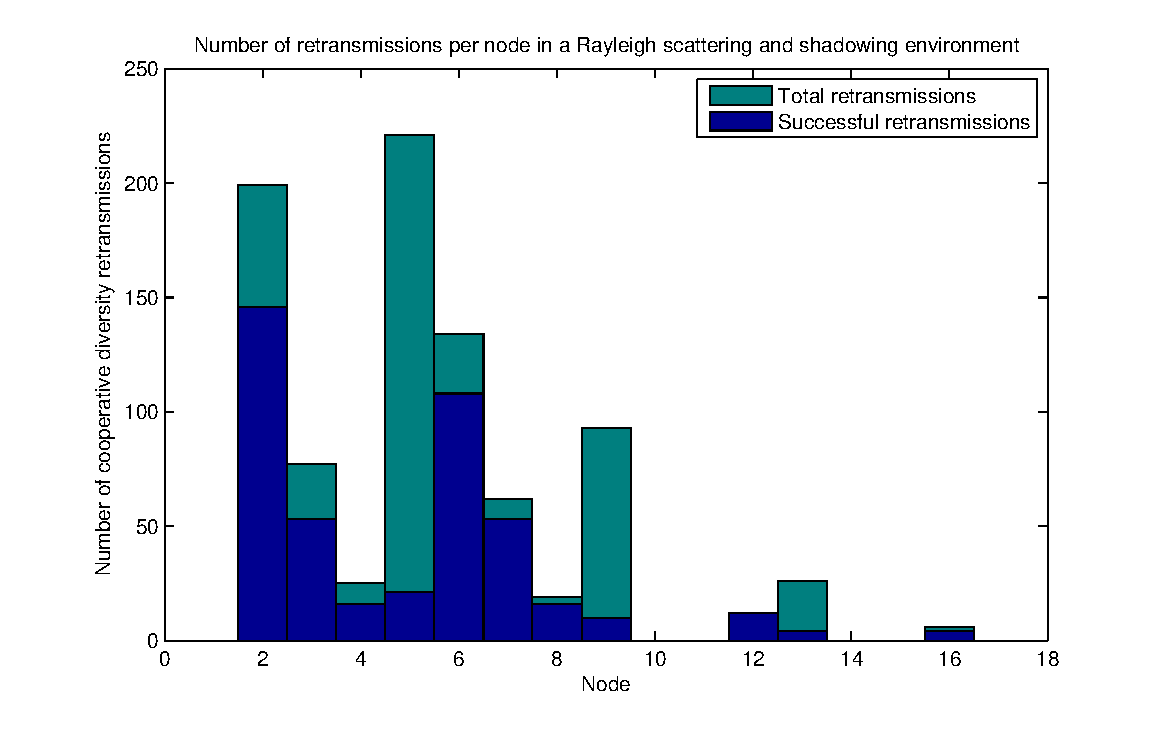
\includegraphics[scale=1]{figures/histogram}
\caption{Histogram of retransmissions at each node in a network.}
\label{fig:histogram}
\end{figure*}
\begin{algorithm}
\caption{Algorithm for selecting diversity nodes by transmission likelihood}          
\label{alg1}
Let $N$ be the set of all other nodes in the ad-hoc network.\\
Let $Q$ be the subset of $N$ that passed the CRC.\\
Let $Q'$ be the subset of $Q$ that has the highest probability of success as a diversity node.\\
Let $P_{ij}$ be the likelihood of transmission to node $j$ if node $i$ is selected as the diversity node.
\begin{algorithmic}                    % enter the algorithmic environment
	\FORALL{$i,j \in N$}
		\STATE Initially assume all nodes have perfect transmission likelihood.
		\STATE $P_{ij} \leftarrow 1$
		\STATE $n_{ij} \leftarrow 1$
	\ENDFOR
    \LOOP
    	\STATE Transmit without diversity from $i$ to $j$.
    	\IF{\{$j$ passes CRC\}}
    		\STATE Send next packet.
    	\ELSE
    		\STATE Let $Q = \{ a \mid \forall a \in N, a $ passes CRC$\}$
			\STATE Let $Q' = \{ b \mid \forall b,c \in Q, P_{bj} \geq P_{cj}\}$
			\IF{$|Q'| > 1$}
				\STATE $m \sim U(1, |Q'|)$
				\STATE $k \leftarrow Q'_m$
			\ELSE
				\STATE $k \leftarrow Q'_1$
			\ENDIF
			\STATE Retransmit from $i$ to $j$ with $k$ selected as diversity node.
			\IF{\{$j$ passes CRC\}}
				\STATE $P_{kj} \leftarrow \frac{P_{kj} n_{kj} + 1}{n_{kj} + 1}$
    			\STATE Send next packet.
    		\ELSE
    			\STATE $P_{kj} \leftarrow \frac{P_{kj} n_{kj}}{n_{kj} + 1}$
    			\STATE Requeue packet for retransmission without diversity.
    		\ENDIF
    	\ENDIF
	\ENDLOOP
\end{algorithmic}
\end{algorithm}

\section{Simulation Results}
Using the 4x4 network, we tested the effects of shadowing on the direct transmission path between the source and destination nodes (Figure \ref{fig:4x4topologyshadowing}), as well as between possible diversity nodes, leaving the direct transmission channel unobstructed (Figure \ref{fig:4x4topology}).
We then compared the throughput of direct transmission to our cooperative diversity scheme in both situations.

Figures \ref{fig:4x4throughput} and \ref{fig:4x4throughputshadowing} display the improvement in throughput using the cooperative diversity scheme compared to direct transmission in the scenarios with and without line of sight from the source to the destination, respectively.
The effective throughput displays a significant increase in both scenarios.
In the scenario with significant shadowing in the direct transmission path, the bandwidth utilization is increased from almost 0\% to roughly half of that of the direct transmission with no shadowing.
This is a fair representation of the improvement this scheme could bring to a system where the channel between two communicating nodes contains significant shadowing.
In addition, the maximum likelihood diversity node selection method shows significant throughput gains in both scenarios.  This can be attributed the the non-selection of nodes with poor channels to the destination node due to distance and shadowing.
\begin{figure}
	\centering
	\begin{subfigure}{}
		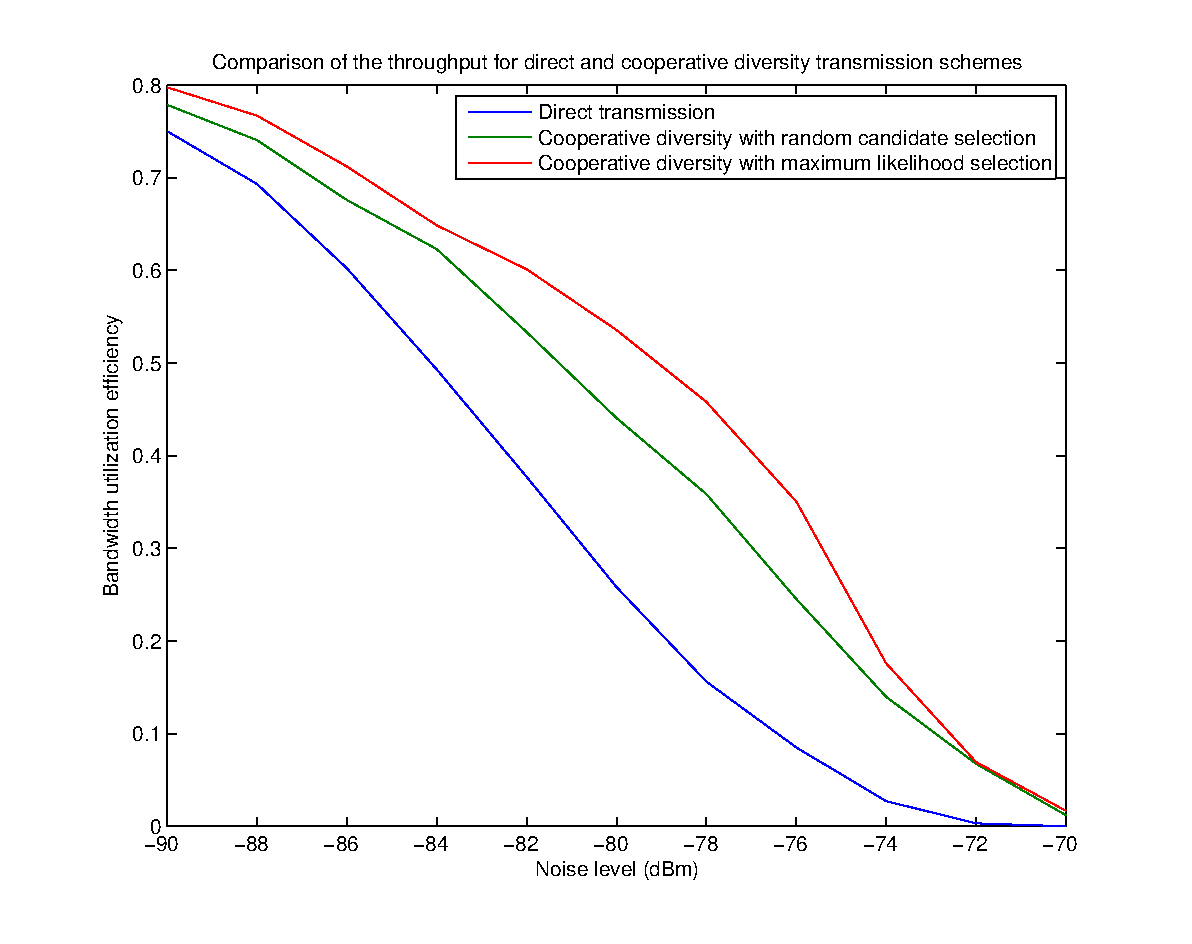
\includegraphics[scale=.45]{figures/4x4throughput}
		\caption{Bandwidth utilization of the 4x4 configuration with line of sight.}
		\label{fig:4x4throughput}
	\end{subfigure}
	
	\vspace{2cm}
	
	\begin{subfigure}{}
		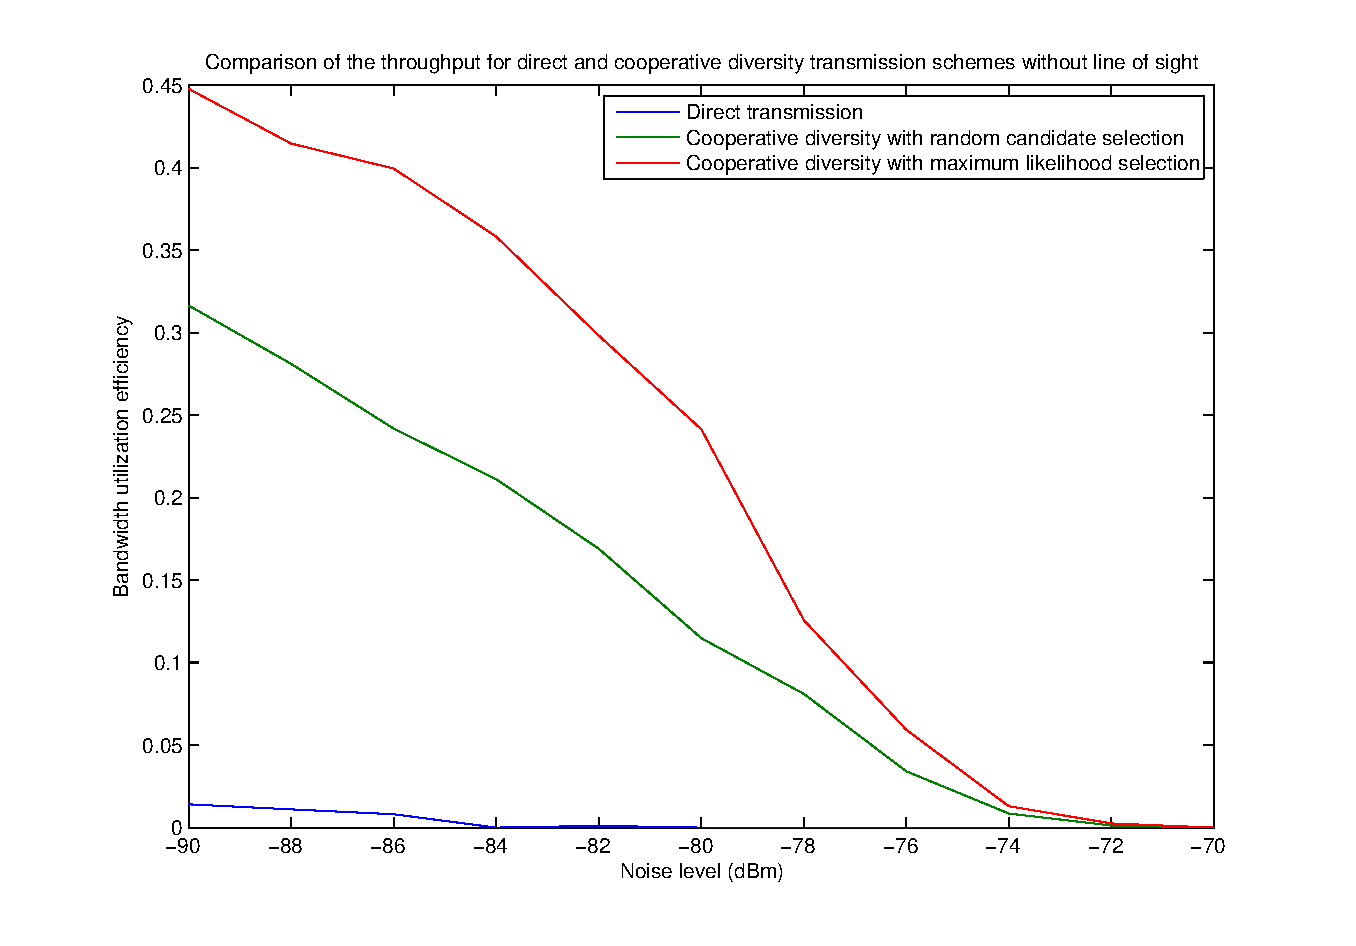
\includegraphics[scale=.4]{figures/4x4throughput_shadowing}
		\caption{Bandwidth utilization of the 4x4 configuration with direct path shadowing.}
		\label{fig:4x4throughputshadowing}
	\end{subfigure}
\end{figure}

In the case of line of sight between the source and destination nodes, cooperative diversity introduces a significant diversity gain in medium to low SNR environments that reduces to an array gain in higher SNR environments.
If nodes expect to have line of sight to other nodes, nodes in the network can disable cooperative diversity in the case of high SNR to decrease the total power consumption of the network without sustaining a significant throughput penalty.
In the case of shadowing in the direct transmission path, this is not the case.
The throughput does not so much depend on the SNR as much as the severe path loss due to the shadowing.
Implementing cooperative diversity in this scenario functions similarly to relaying the data, without the complexity of identifying the source of data loss as poor channel state or shadowing.
In the shadowing example, the benefit of cooperative diversity grows with increasing SNR, but may not be as efficient as a pure relaying scheme.

These simulation results show that cooperative diversity is an effective method of increasing throughput in both shadowing and low SNR environments without the need of identifying the source of data loss.

\section{Conclusion}
In this paper, a relatively low complexity method of obtaining transmitter-side diversity gain in an ad-hoc network by use of cooperative diversity without necessitating antenna diversity at any node was simulated.
The source node transmitted packets along with a CRC allowing for low complexity selection of cooperative diversity candidate nodes at the transport layer without any explicit knowledge of channel state at any other nodes.
If the destination node failed the CRC, a candidate was selected to retransmit the packet along with the source node using Alamouti's rate 1 space-time block code.
This method proved to significantly increase throughput.
In addition, intelligent selection of candidate nodes based on maximum likelihood of successful transmission further increased the throughput gains of this system.
Overall, cooperative diversity was shown to be an effective method of increasing throughput in ad-hoc networks.

\nocite{*}
\bibliographystyle{ieeetran}
\bibliography{IEEEabrv,sections/references}

\end{document}


